%% Paquetes y configuración %

% Beamer
\PassOptionsToPackage{unicode}{hyperref}  % Evita errores con caracteres no ASCII
\PassOptionsToPackage{naturalnames}{hyperref} % tex.stackexchange.com/questions/10555
\documentclass[compress]{beamer}

% Idioma
\usepackage[spanish]{babel} % Traducciones
\usepackage[utf8]{inputenc} % Uso de caracteres UTF-8
\usepackage{lmodern}        % Fuentes de tamaño arbitrario
\usepackage[T1]{fontenc}    % Permite copiar y evita errores
\uselanguage{Spanish}       % Traducciones beamer
\languagepath{Spanish}      % (tex.stackexchange.com/questions/168208)

% Matemáticas
\usepackage{amsfonts}
\usepackage{amsmath}
\usepackage{amssymb}

% Colores
\definecolor{backg}{HTML}{F2F2F2}    % Fondo
\definecolor{title}{HTML}{bdc3d1}    % Títulos
\definecolor{comments}{HTML}{BDBDBD} % Comentarios
\definecolor{keywords}{HTML}{08388c} % Palabras clave
\definecolor{strings}{HTML}{FA5858}  % Strings
\definecolor{links}{HTML}{2C2C95}    % Enlaces
\definecolor{bars}{HTML}{045FB4}     % Barras (gráfico)

% Código
\usepackage{listings}
\lstset{
language=[LaTeX]TeX,
basicstyle=\footnotesize,
morekeywords={href,uselanguage,languagepath,column},
otherkeywords={pause,usetheme,usecolortheme,useinnertheme,titlepage,tableofcontents,subtitle},
breaklines=true,
backgroundcolor=\color{backg},
keywordstyle=\color{keywords},
commentstyle=\color{comments},
stringstyle=\color{strings},
tabsize=2,
% Acentos, ñ, ¿, ¡ (tex.stackexchange.com/questions/24528)
extendedchars=true,
literate={á}{{\'a}}1 {é}{{\'e}}1 {í}{{\'i}}1 {ó}{{\'o}}1
         {ú}{{\'u}}1 {ñ}{{\~n}}1 {¡}{{\textexclamdown}}1
         {¿}{{?`}}1
}

% Gráficos
\usepackage{pgfplots}
\pgfplotsset{width=7cm,compat=1.8} % Opciones para gráficos

% Columnas
\usepackage{multicol}

% Emoticonos
\usepackage{wasysym}

% tikz
\usepackage{tikz}
\usetikzlibrary{mindmap,trees,shadows}
\tikzset{ % Genera overlays
    invisible/.style={opacity=0},
    visible on/.style={alt={#1{}{invisible}}},
    alt/.code args={<#1>#2#3}{\alt<#1>{\pgfkeysalso{#2}}{\pgfkeysalso{#3}}},
}
\usepackage{gnuplot-lua-tikz}

%% Comandos %%
\newcommand{\ejemplo}[1]{\lstinputlisting{./examples/#1}} % Mostrar código de ejemplos
\newcommand{\muestra}[1]{\input{./examples/#1}}           % Mostrar ejemplos
\newcommand{\seccion}[1]{\input{./sections/#1}}           % Incluir secciones
\newcommand{\espacio}{\vspace*{\baselineskip}}            % Añade espacios
\newcommand{\beamer}{\texttt{beamer} }                    % Estilo único para beamer
\newcommand{\enlace}[3]{\href{#1}{\textbf{#2}} - {\small #3}}  % Estílo único para refs
\newcommand{\comando}[1]{{\color{black}\textbackslash}{\color{keywords}#1}}

%% Temas %%
% Tema y tema de color
  \usetheme{Szeged}
  \usecolortheme{crane}
% \useinnertheme{circles}
  \setbeamercovered{transparent}
% Colores bloques
%  \setbeamercolor{block title}{bg=title,fg=links}
%  \setbeamercolor{block body}{bg=backg,fg=black}
%  \setbeamercolor{block title alerted}{fg=red!70!black,bg=title!92!red}
%  \setbeamercolor{block body alerted}{fg=black,bg=backg}
%  \setbeamercolor{block title example}{fg=green!70!black,bg=title!92!green}
%  \setbeamercolor{block body example}{fg=black,bg=backg}
% Enlaces (tex.stackexchange.com/questions/13423)
\hypersetup{colorlinks,linkcolor=,urlcolor=links}
% Quita enlaces de navegación (stackoverflow.com/questions/3017030)
\setbeamertemplate{navigation symbols}{}
% Quita barra inferior (stackoverflow.com/questions/1435837)
\setbeamertemplate{footline}{}
% Evita warnings boxes
\hfuzz=20pt
\vfuzz=20pt
% Evita wranings itemize
\renewcommand\textbullet{\ensuremath{\bullet}}
\definecolor{naranja}{RGB}{252,187,6}
\definecolor{verde}{RGB}{64,159,64}

% tikz
\usepackage{tikz}
\usetikzlibrary{shapes.multipart}

%% Título y otros %%
\title{Presentación práctica Backtracking y Branch and Bound}                                               % Título
\subtitle{Asignatura: Algorítmica}                                  % Subtítulo
\author{Rubén Morales Pérez
		\and Francisco Javier Morales Piqueras
		\and Bruno Santindrian Manzanedo
		\and Ignacio de Loyola Barragan Lozano
		\and Francisco Leopoldo Gallego Salido}
\date{\today}                                                            % Fecha


%%%%%%%%%%%%%%%%%%%%%%%%%%%%%%%%%%%%%%%%%%%%%%%%%%%%%%%%%%%%%%%%

%% Presentación %%
\begin{document}

\begin{frame}
\titlepage
\end{frame}
\begin{frame}{Índice}
  \hypertarget{index}{}
  \tableofcontents
\end{frame}

\section{División en dos equipos}
\subsection{Enunciado}
\begin{frame}{Enunciado}
	\begin{block}{Equipos}
		Se desea dividir un conjunto de $n$ personas para formar dos equipos que competirán entre sí.
		Cada persona tiene un cierto nivel de competición, que viene representado por una puntuación 
		(un valor numérico entero). Con el objeto de que los dos equipos tengan un nivel similar, se
		pretende construir los equipos de forma que la suma de las puntuaciones de sus miembros sea 
		lo más similar posible. Diseña e implementa un algoritmo vuelta atrás para resolver este
		problema. 
	\end{block}
\end{frame}

\begin{frame}{Puntuación de cada jugador}
	\begin{block}{Nivel individual}
	Tenemos $n$ jugadores con puntuación respectiva $x_i\ \forall i\in I=[1, 1000]\cap \mathbb{N}$.
	Identificamos a cada jugador única y exlusivamente por su puntuación.
	\end{block}
	
	\begin{alertblock}{¿Problema?}
	Esto permite que si hay dos jugadores con nivel de competición $x$ e $y$ con $x=y$ y cada uno 
	está en un equipo podrían intercambiar sus posiciones sin descompensar los equipos.	
	Así obtenemos una mayor flexibilidad, por si queremos tener en cuenta factores de compenetración
	entre los jugadores dependiendo del equipo en el que estén.
	\end{alertblock}
\end{frame}

\begin{frame}{Rango inicial diferente}
	\begin{block}{ }
	Si inicialmente tuviésemos los niveles de los jugadores en otro rango $J=[a, b]\ a,b\in\mathbb{N}: 
	a<b$ podemos dejarlo así, ya que el rango de los niveles no afecta al problema.
	\end{block}
	
	\begin{exampleblock}{Excepción}
 	Si aplicamos una transformación que reduzca el rango, podríamos perder información al aproximar a 	
 	números	enteros, ya que el enunciado pide que sean números enteros.	
	\end{exampleblock}
\end{frame}


\begin{frame}
	\begin{block}{Transformación}
	En cualquier caso la transformación al dominio del problema (números naturales dentro de $I$) 
	del intervalo $J$ es: $\forall j\in J$ aplicamos una función $F:[a,b] \rightarrow
	[1,1000]\cap\mathbb{N}$
	\end{block}
	
	\begin{exampleblock}	{Función $E(x)$}
	Teniendo en cuenta que $E(x)$ es la función parte entera:
	\end{exampleblock}
	
	\begin{exampleblock}{Fórmula}
	\[F(x) = \left\{
	\begin{matrix}
		E\left( \frac{x-a}{b-a}\cdot 1000 \right)+1  & 
		\mbox{si } \frac{x-a}{b-a}\cdot 1000 < 
					E\left( \frac{x-a}{b-a}\cdot 1000 \right) + \frac{1}{2}

	 \\	E\left( \frac{x-a}{b-a}\cdot 1000 \right)    & 
	 	\mbox{en otro caso}
	\end{matrix}
	\right.\]
	\end{exampleblock}
\end{frame}

\subsection{Eficiencia}
\begin{frame}
	\begin{block}{Desarrollo}
	Tomando el primer jugador, puede estar en un equipo o en otro, $2$ combinaciones. 
	Cogemos el siguiente jugador, puede estar en uno u otro, independientemente de donde 
	estuviese el anterior, $2^2$ combinaciones. 
	El tercer jugador vuelve a tener $2$ opciones independientes del resto, $2^3$ combinaciones. 	
	
	Tenemos que pasar por todas las opciones, por tanto la eficiencia del algoritmo es $O(n)=2^n$
	\end{block}
	
	\begin{block}{Representación}
	Podemos representar el problema como un vector de bool de $n$ elementos. Si un jugador está
	en el primer equipo el valor será \textit{true}, en caso contrario será \textit{false}.
	\end{block}
\end{frame}

\begin{frame}
	\begin{columns}
	\column	{.35\textwidth}
	Al tratarse de un algoritmo de vuelta atrás (backtraking) tenemos que recorrer todas las 
	opciones, por lo que el problema queda representado como un árbol binario donde cada nodo 
	tiene dos opciones, estar en un equipo o en otro.
	
	\column	{.65\textwidth}
	\begin{figure}[H]
    		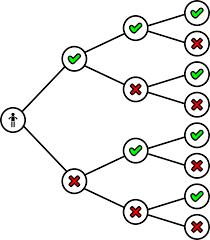
\includegraphics[scale=0.65]{./Imagenes/arbolbin.png}
	\end{figure}		
	\end{columns}
\end{frame}


\begin{frame}{Otra versión}
	\begin{block}{Mejora}
	Forzaremos que la diferencia de jugadores entre ambos equipos no sea mayor de $1$. 
	Si hay un número $n$ par los equipos tendrán el mismo número de jugadores. 
	El algoritmo sigue teniendo eficiencia $O(n)=2^n$ ya que pasaremos por todas las opciones, pero
	cuando una combinación no cumpla dicha restricción no haremos sus cálculos asociados.	
	\end{block}

	\begin{alertblock}{Ajustes}
	EL rango usado ha sido $I=[3,26]\cap\mathbb{N}$.
	Hemos ajustado funciones $f(n)=a \cdot 2^n\ a\in\mathbb{R}	\ \forall n\in I$. 
	Sus coeficientes $r^2$ son $1$ en ambos casos (hay pocos elementos) y el 	
	término $a$ está especificado en las gráficas.
	\end{alertblock}
\end{frame}


\subsection{Comparando ambos algoritmos}
\begin{frame}
	\begin{exampleblock}{Sin equilibrio de jugadores}
	\begin{figure}[H]
    		\centering
   		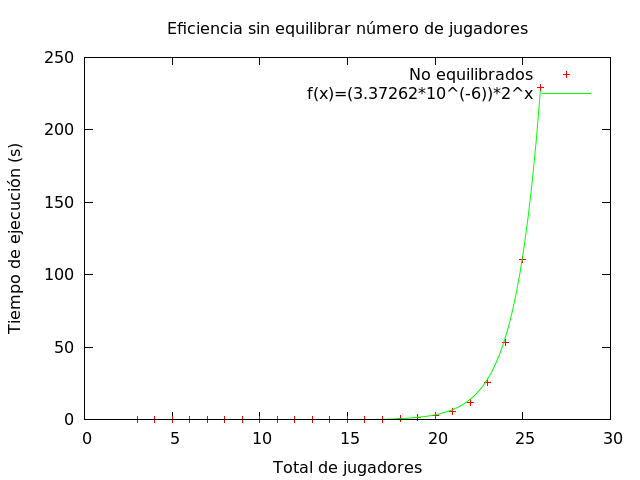
\includegraphics[scale=0.4]{../Equipos/Graficas/sinEquilibrar.png}
    		\label{fig:Sin equilibrar}
	\end{figure}
	\end{exampleblock}
\end{frame}

\begin{frame}
	\begin{exampleblock}{Equilibrando jugadores}
	\begin{figure}[H]
    		\centering
	    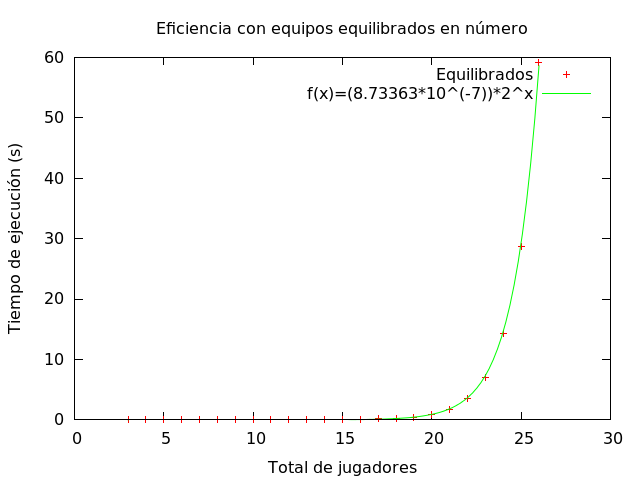
\includegraphics[scale=0.4]{../Equipos/Graficas/equilibrar.png}
    		\label{fig:Equilibrado}
	\end{figure}
	\end{exampleblock}
\end{frame}

\begin{frame}
	\begin{exampleblock}{Comparando tiempo}
	\begin{figure}[H]
    		\centering
	    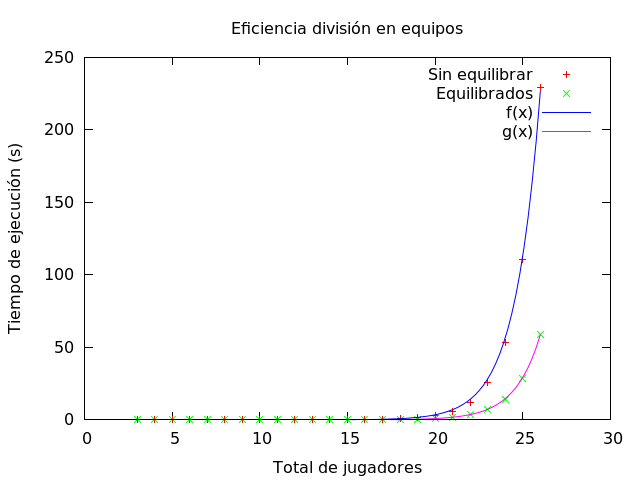
\includegraphics[scale=0.4]{../Equipos/Graficas/tiempos.png}
    		\label{fig:divisionTiempos}
	\end{figure}
	\end{exampleblock}
\end{frame}

\begin{frame}
	\begin{block}{Nivel}
	Recordemos que un jugador tiene un nivel entre $1$ y $1000$, es lógico pensar que con pocos 
	jugadores el margen de optimización del algoritmo es menor debido al gran peso que toma la
	aleatoriedad con la que se determinan los niveles.
	\end{block}
	
	\begin{block}{Tendencia}
	El primer algoritmo tiende a desajustar el número de jugadores, llegando a tener los equipos 
	una diferencia de $4$ jugadores cuando siendo $24$ en total.
	\end{block}
\end{frame}

\begin{frame}
	\begin{exampleblock}{Diferencia de nivel entre los equipos}
		\begin{figure}[H]
    		\centering
    		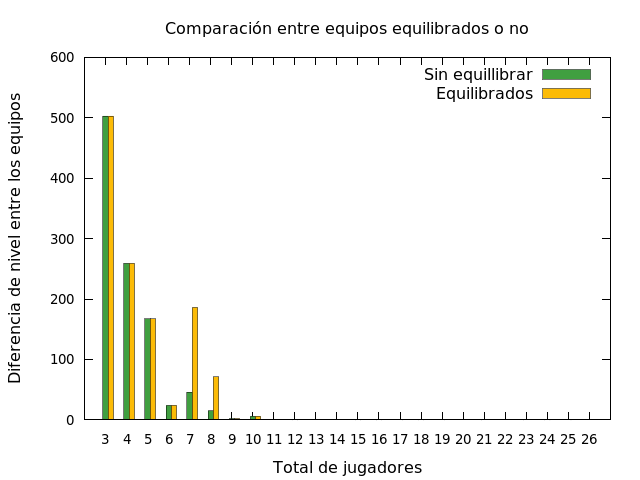
\includegraphics[scale=0.4]{../Equipos/Graficas/comparativa.png}
    		\label{fig:comparativa}
	\end{figure}
	\end{exampleblock}
\end{frame}

\begin{frame}
	\begin{exampleblock}{Número de jugadores de diferencia}
	\begin{figure}[H]
    		\centering
    		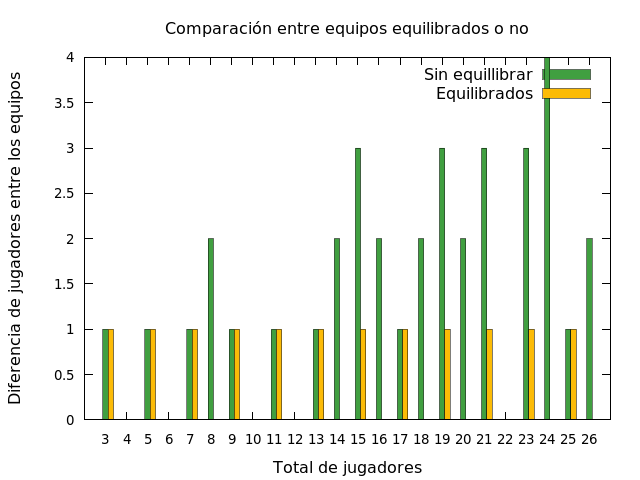
\includegraphics[scale=0.4]{../Equipos/Graficas/separacion.png}
    		\label{fig:separacion}
	\end{figure}
	\end{exampleblock}
\end{frame}

\subsection{Conclusión}
\begin{frame}
	\begin{block}{Opciones}
	Para ejecuciones con un número pequeño de elementos los algoritmos planteados nos sirven, 
	pero si aumentamos el número esa fuerza bruta no es tan buena idea.
	
	Opciones:
	\begin{itemize}
		\item Poda el árbol: ``Branch and Bound".
		\item $x,y$ nivel de los equipos, conformarnos con $|x-v|<n\in\mathbb{N}$
		\item Paralelismo, cada procesador comprueba una rama
	\end{itemize}
	\end{block}
	
	\pause
	\begin{alertblock}{Conclusión}
	Como hemos comprobado, el segundo algoritmo iguala al primero en eficacia, pero lo supera
	en eficiencia.
	Esto nos hace pensar que puede no ser necesario siempre recorrer todo el árbol de soluciones 
	para asegurarnos la optimalidad.
	\end{alertblock}
\end{frame}

\section{Viajante de comercio}
\subsection{Enunciado}
\begin{frame}
	\begin{block}{Viajante de comercio con vuelta atrás y ramificación y poda}
	Cuando para un nivel no queden más ciudades válidas, el algoritmo hace una vuelta atrás 
	proponiendo una nueva ciudad válida para el nivel anterior.

	Para el algoritmo de ramificación y poda es necesario utilizar una cota inferior para cada nodo 
	(solución parcial), un valor $c$ menor o igual que el verdadero coste de la mejor solución (la de 
	menor coste) que se puede obtener a partir de la solución parcial en la que nos encontremos.

	Para realizar la poda, guardamos en todo momento en una variable $C$ el costo de la mejor solución
	obtenida hasta ahora, si para una solución parcial, $c>C$ entonces se puede podar.

	Como criterio para seleccionar el siguiente nodo vivo se empleará el criterio LC o 
	``más prometedor", aquel que presente el menor valor de cota inferior.
	\end{block}
\end{frame}


\subsection{Explicación}
	
\begin{frame}
Hemos utilizado dos algoritmos para encontrar una cota inferior.
	
	\begin{block}{Algoritmo propuesto}
	Para encontrar la longitud del grafo con los menores arcos sumamos el menor elemento de cada fila de la matriz de adyacencia.
	\end{block}
	
	\begin{alertblock}{Problema}
	En matrices simétricas podemos repetir elementos simétricos y acabar con un grafo inconexo.
	\end{alertblock}
	
	\begin{block}{Algoritmo mejorado}
	Si hemos usado el simétrico de un elemento escogemos el siguiente menor.
	\end{block}
\end{frame}

\begin{frame}{Ejemplo}
\begin{columns}
\begin{column}{5cm}
	\[
	\begin{bmatrix}
	    0 & 1 & 2 & 3\\
	    1 & 0 & 4 & 5\\
	    2 & 4 & 0 & 6\\
	    3 & 5 & 6 & 0\\
	\end{bmatrix}
	\]
\end{column}

\begin{column}{7cm}
	\begin{figure}[H]
    		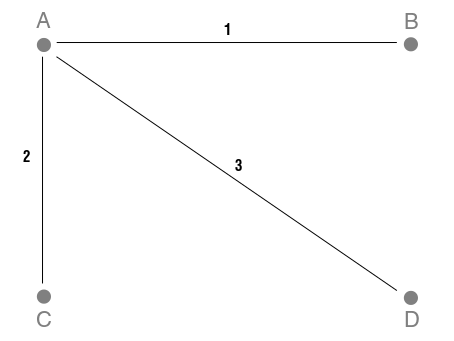
\includegraphics[scale=0.25]{./Imagenes/ej.png}
	\end{figure}
	
	\begin{figure}[H]
	    		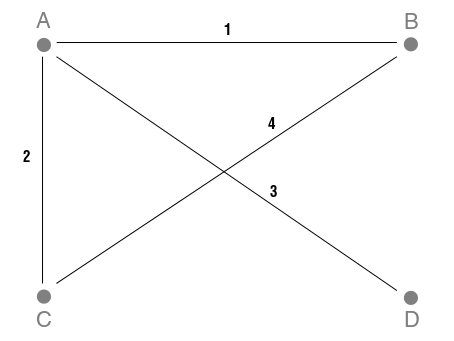
\includegraphics[scale=0.25]{./Imagenes/ej_mejorado.png}
	\end{figure}
\end{column}
\end{columns}
\end{frame}


\subsection{Eficiencia}
\begin{frame}
	\begin{block}{Eficiencia recorriendo el arbol}
	Tenemos que evaluar las permutaciones de un conjunto de $n-1$ elementos, por tanto la eficiencia será $O(n!)$.
	\end{block}
	
	\begin{block}{Eficiencia de la primera cota}
		Recorremos los elementos de todas las filas. Por tanto $O(n^2)$.
	\end{block}
	
	\begin{block}{Eficiencia de la segunda cota}
		Como sabemos en que fila se encuentra el simétrico de cualquier elemento y solo guardamos un elemento por fila, la comprobación es $O(1)$ y el algoritmo $O(n^2)$.
	\end{block}

\end{frame}





\subsection{Recorridos}

\begin{frame}
	\begin{exampleblock}{Imagen}
	\begin{figure}[H]
    	\centering
    	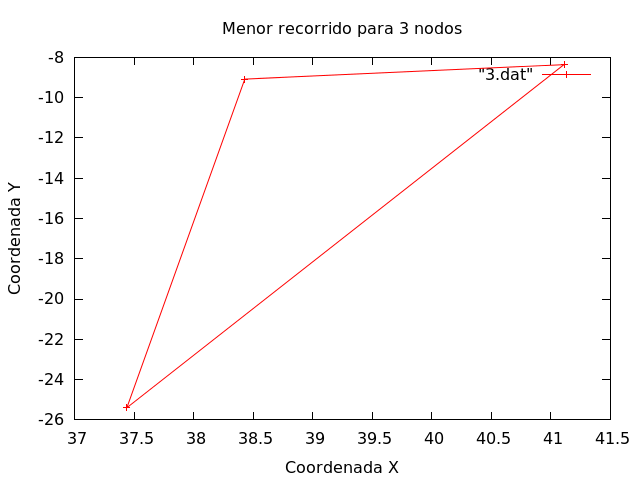
\includegraphics[scale=0.35]{../TSP/Graficas/3.png}
	\end{figure}
	\end{exampleblock}
\end{frame}

\begin{frame}
	\begin{exampleblock}{Imagen}
	\begin{figure}[H]
    	\centering
    	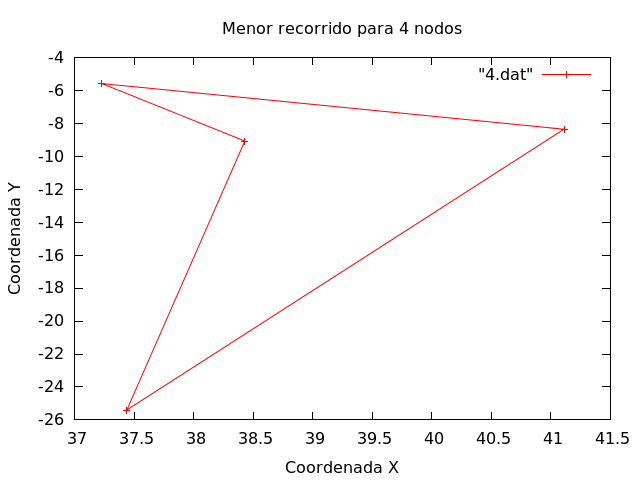
\includegraphics[scale=0.35]{../TSP/Graficas/4.png}
	\end{figure}
	\end{exampleblock}
\end{frame}

\begin{frame}
	\begin{exampleblock}{Imagen}
	\begin{figure}[H]
    \centering
    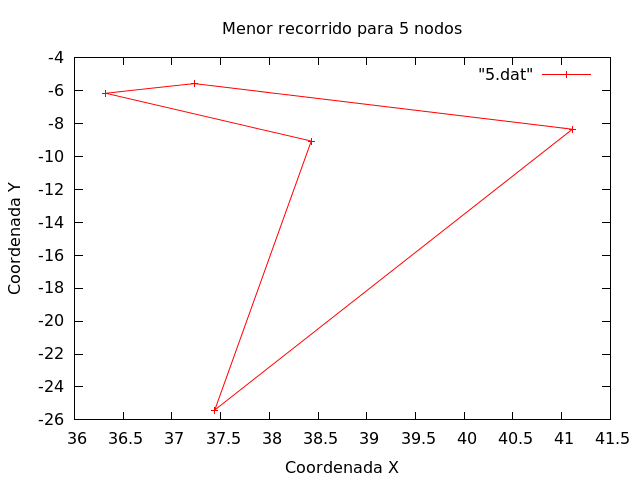
\includegraphics[scale=0.35]{../TSP/Graficas/5.png}
	\end{figure}
	\end{exampleblock}
\end{frame}

\begin{frame}
	\begin{exampleblock}{Imagen}
	\begin{figure}[H]
    \centering
    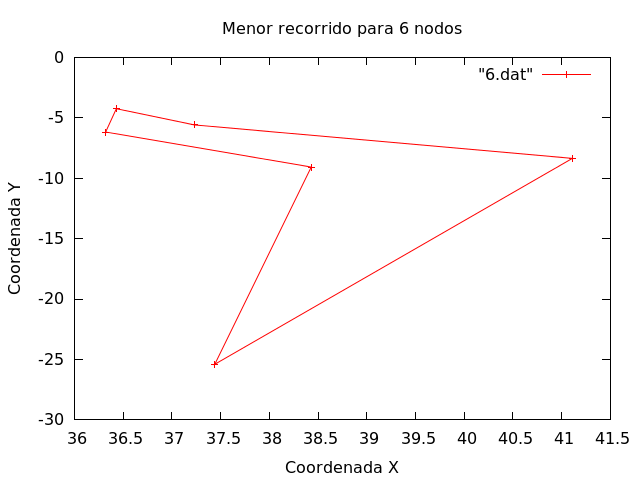
\includegraphics[scale=0.35]{../TSP/Graficas/6.png}
	\end{figure}
	\end{exampleblock}
\end{frame}

\begin{frame}
	\begin{exampleblock}{Imagen}
	\begin{figure}[H]
    \centering
    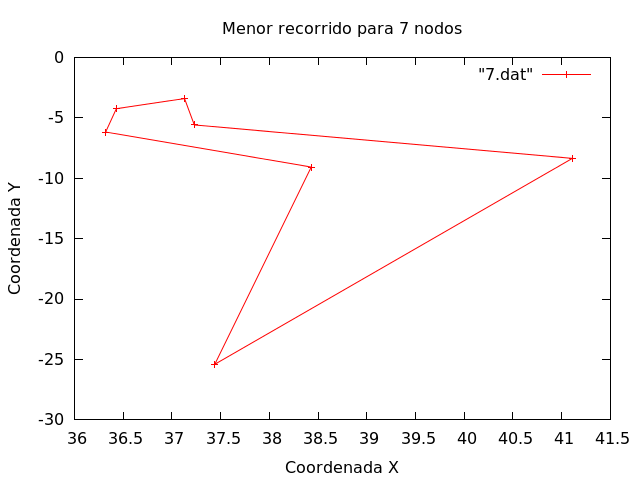
\includegraphics[scale=0.35]{../TSP/Graficas/7.png}
	\end{figure}
	\end{exampleblock}
\end{frame}

\begin{frame}
	\begin{exampleblock}{Imagen}
	\begin{figure}[H]
    \centering
    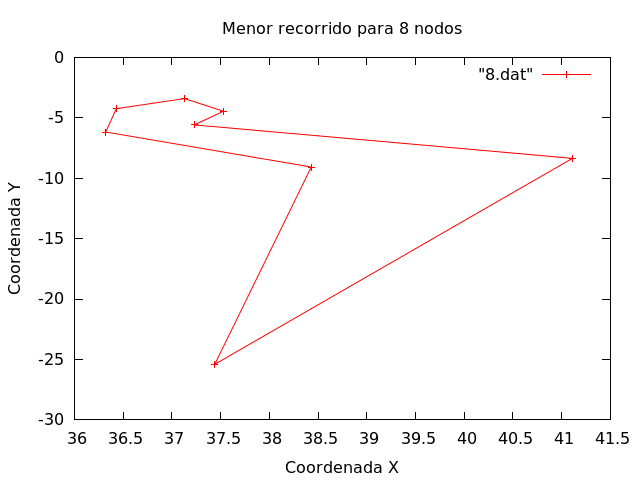
\includegraphics[scale=0.35]{../TSP/Graficas/8.png}
	\end{figure}
	\end{exampleblock}
\end{frame}

\begin{frame}
	\begin{exampleblock}{Imagen}
	\begin{figure}[H]
    \centering
    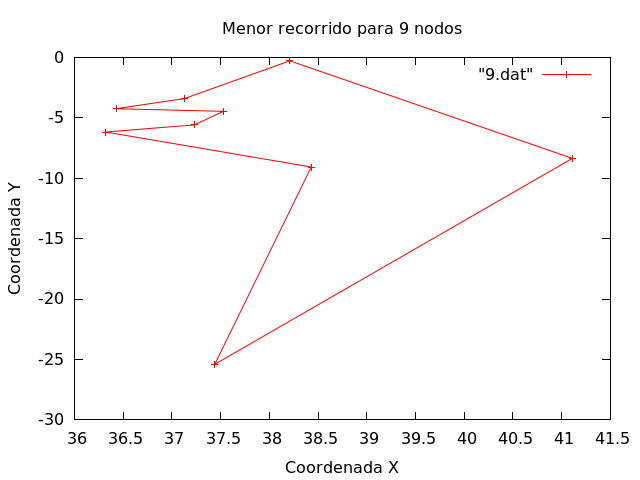
\includegraphics[scale=0.35]{../TSP/Graficas/9.png}
	\end{figure}
	\end{exampleblock}
\end{frame}

\begin{frame}
	\begin{exampleblock}{Imagen}
	\begin{figure}[H]
    \centering
    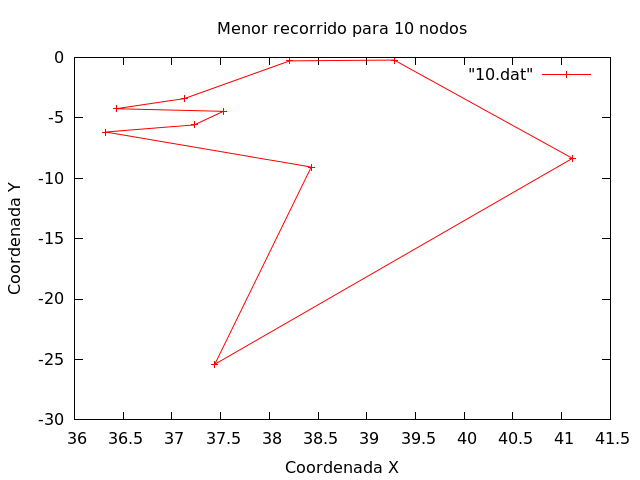
\includegraphics[scale=0.35]{../TSP/Graficas/10.png}
	\end{figure}
	\end{exampleblock}
\end{frame}

\begin{frame}
	\begin{exampleblock}{Imagen}
	\begin{figure}[H]
    \centering
    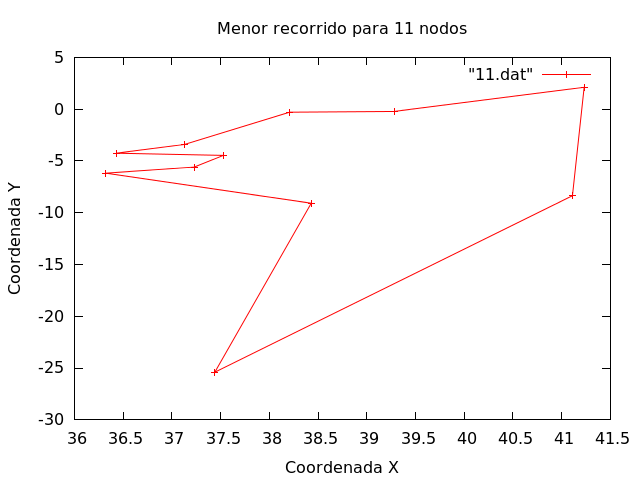
\includegraphics[scale=0.35]{../TSP/Graficas/11.png}
	\end{figure}
	\end{exampleblock}
\end{frame}

\begin{frame}
	\begin{exampleblock}{Imagen}
	\begin{figure}[H]
    \centering
    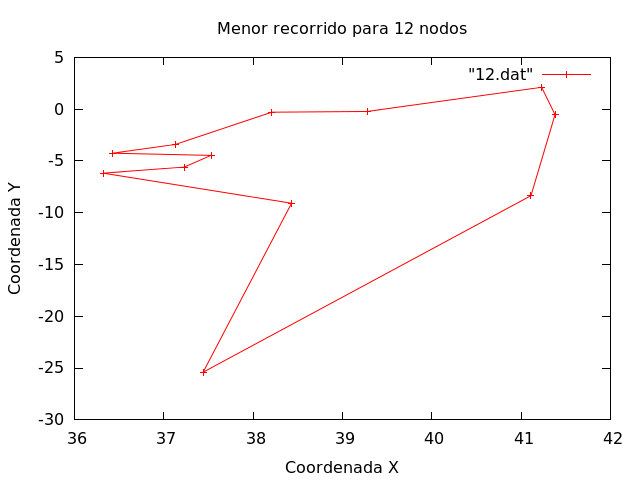
\includegraphics[scale=0.35]{../TSP/Graficas/12.png}
	\end{figure}
	\end{exampleblock}
\end{frame}

\begin{frame}
	\begin{exampleblock}{Imagen}
	\begin{figure}[H]
    \centering
    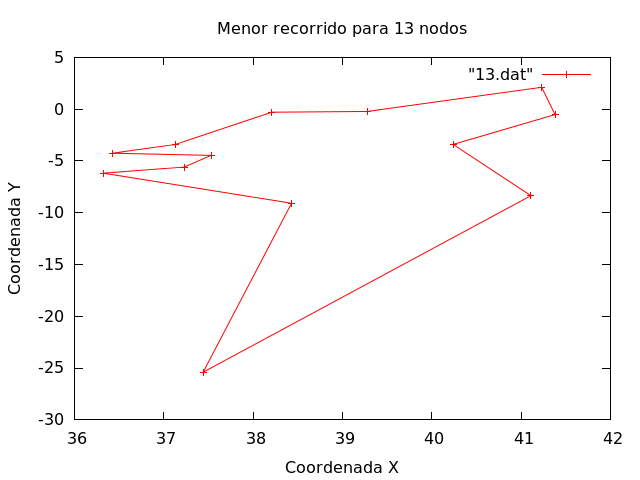
\includegraphics[scale=0.35]{../TSP/Graficas/13.png}
	\end{figure}
	\end{exampleblock}
\end{frame}




\subsection{Comparativa}
\begin{frame}{Comparativa}
	\begin{block}{Funciones de cota}
	Las diferentes funciones para conseguir una cota inferior hacen que en un mismo mapa
	el algoritmo de ramificación y poda varíe. 
	\end{block}
	
	\begin{exampleblock}{Datos}
	\begin{itemize}
		\item Nodos expandidos
		\item Mayor cola de nodos vivos
		\item Cantidad de cortes
		\item Tiempo
	\end{itemize}
	\end{exampleblock}
\end{frame}



\subsubsection{Cortes producidos}
\begin{frame}{Cortes}
	\begin{block}{Representatividad}
	Esta información puede no ser representativa de la
	magnitud de los cortes. Dados dos algoritmos $X,Y$ que han hecho $x_i,y_i$ cortes
	respectivamente con $x_1>y_1$ no nos está diciendo que el primero sea más rapido.
	El primer algoritmo podría haber recorrido más nodos y hacer los cortes en niveles 
	del árbol más profundos. 
	\end{block}
\end{frame}
 
\begin{frame}
	\begin{exampleblock}{Imagen}
	\begin{figure}[H]
    		\centering
	    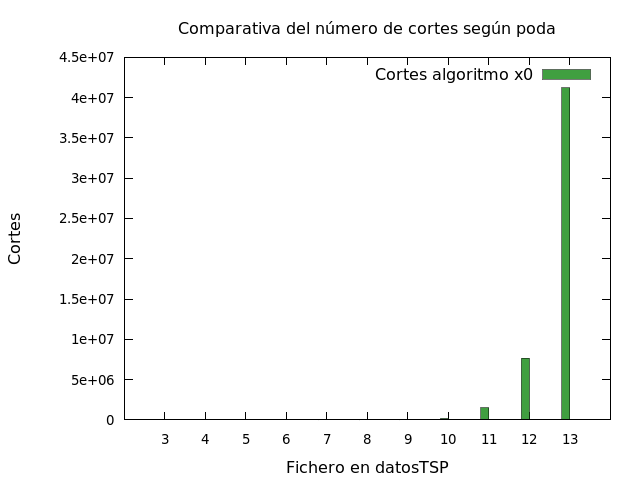
\includegraphics[scale=0.35]{../TSP/Graficas/graficaCortes.png}
    		\caption{Cortes efectuados}
	\end{figure}
	\end{exampleblock}
\end{frame}



\subsubsection{Colas con prioridad}
\begin{frame}{Tamaño de la lista de nodos vivos}
	\begin{block}{ }
	A continuación exponemos el mayor tamaño alcanzado por la cola con prioridad.
	Esta información nos puede dar una idea de lo bueno que es nuestro algoritmo 
	para el cálculo de una cota inferior.
	\end{block}
	
	\begin{block}{Otras versiones}
	Hay versiones de ramificación y poda para el problema del viajante
	de comercio que no usan por ejemplo la aproximación greedy inicial, por lo que ha podido 
	sobrecargar la cola con prioridad mientras busca la primera solución con la que podará después.
	\end{block}
\end{frame}

\begin{frame}
	\begin{exampleblock}{Imagen}
	\begin{figure}[H]
    		\centering
	    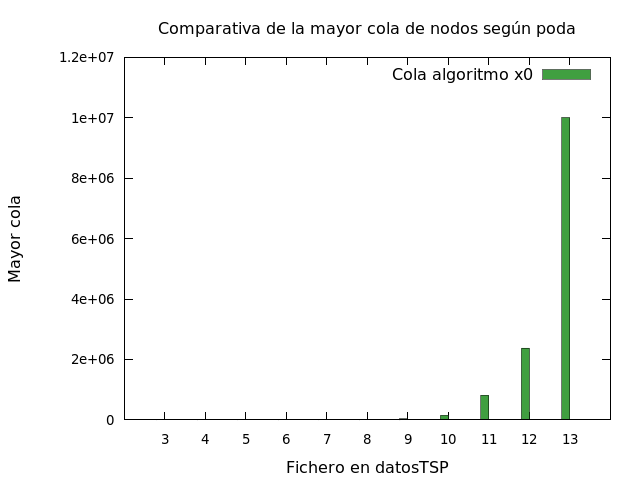
\includegraphics[scale=0.35]{../TSP/Graficas/graficaColaMaxima.png}
    		\caption{Cola con prioridad más grande}
	\end{figure}
	\end{exampleblock}
\end{frame}


\subsubsection{Nodos procesados}
\begin{frame}{Nodos}
	\begin{block}{Utilidad}
	Este dato no nos asegura que tarde menos tiempo, ya que un algoritmo con más nodos 
	expandidos que otro ha podido usar una función para calcular las cotas inferiores demasiado costosa.
	\end{block}
\end{frame}

\begin{frame}
	\begin{exampleblock}{Imagen}
	\begin{figure}[H]
    		\centering
	    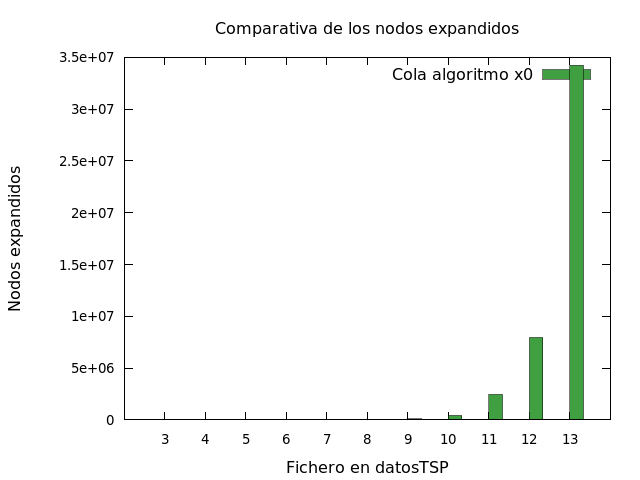
\includegraphics[scale=0.35]{../TSP/Graficas/graficaNodos.png}
    		\caption{Nodos expandidos}
	\end{figure}
	\end{exampleblock}
\end{frame}


\subsubsection{Tiempos}
\begin{frame}
	\begin{exampleblock}{Imagen}
	\begin{figure}[H]
    		\centering
	    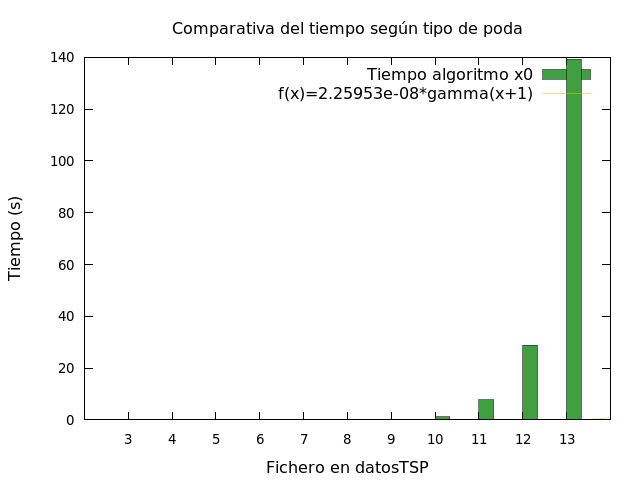
\includegraphics[scale=0.35]{../TSP/Graficas/graficaTiempos.png}
    		\caption{Comparativa de tiempos}
	\end{figure}
	\end{exampleblock}
\end{frame}



\subsection{Conclusión}
\begin{frame}
	\begin{alertblock}{Conclusión}
	Aunque los algoritmos de ramificación y poda nos aseguraran la optimalidad a problemas con
	tiempos de ejecución exponenciales ahorrándonos pasos, no resultan prácticos cuando el tamaño
	del problema crece. Los algoritmos greedy estudiados anteriormente nos pueden dar una 
	aproximación más que razonable para el problema.
	\end{alertblock}
\end{frame}



\end{document}
